\documentclass{article}
\usepackage{amsmath}
\usepackage{amssymb}
\usepackage[a4paper, top=25mm, bottom=25mm, left=25mm, right=25mm]{geometry}
\usepackage{pgfplots}
\usepackage{mathtools}
\pgfplotsset{compat=1.18}
\usepgfplotslibrary{fillbetween}

\begin{document}
\pagestyle{empty}
\large

\begin{center}
2012-2013 Fall \\MAT123-[Instructor02]-02, [Instructor05]-05 Midterm II\\(19/12/2012)\\Time: 09:00 - 11:00\\Duration: 120 minutes
\end{center}

\noindent 1. A 10 m long wire is cut into two pieces. One piece is bent into an equilateral triangle and the other piece is bent into a circle. If the sum of the areas enclosed by each part is minimum, what is the length of each piece?

\hfill

\noindent 2. Integrate the following functions, and write each step in detail.

\hfill

(a) $\displaystyle\int\frac{dy}{\sqrt{y}\left(1+\sqrt y\right)^2}$ \ \ \ (b) $\displaystyle\int_{\pi/6}^{\pi/4}\frac{\cot x}{\ln(\sin x)}\,dx$ \ \ \ (c) $\displaystyle\int\frac{x^3-4x-10}{x^2-x-6}\,dx$

\hfill

\hfill

(d) $\displaystyle \int\tan x \sec^{123}x\,dx$ \ \ \ (e) $\displaystyle\int\sqrt{t-t^2}\,dt$ \ \ \ (f) $\displaystyle\int\sqrt{1+\sqrt x}\,dx$

\hfill

\hfill

\noindent 3. Integrate the following functions, and write each step in detail.

\hfill

(a) $\displaystyle \int_0^2\frac{dx}{\sqrt{|x-1|}}$ \ \ \ (b) $\displaystyle\int_{-\infty}^{\infty}x^2\mathrm{e}^{-x^3}\,dx$

\hfill

\hfill

\noindent 4. By using the Washer Method, find the volume of the solid generated by revolving the region bounded by the curves $x=y^3$ and $y+x^2=0$ about the $x$-axis.

\newpage

\begin{center}
2012-2013 Fall Midterm II (19/12/2012) Solutions\\
(Last update: 29/08/2025 19:47)
\end{center}

\noindent 1. Let $x$ be the length of the wire that is used to form the equilateral triangle. So, $10-x$ is the length of the other piece. The area of the triangle is

\begin{equation*}
A_1 = \frac{x^2\sqrt3}{4}
\end{equation*}

\hfill

\noindent The perimeter of the circle is $10-x$. Therefore, $2\pi r = 10-x$, where $r$ is the radius of the circle. The area of the circle can be extracted from the formula $A_2=\pi r^2$. Solve the former equation for $r$, and express the area in terms of $x$.

\begin{equation*}
    r=\frac{10-x}{2\pi}\,\rightarrow\, A_2 = \pi\left(\frac{10-x}{2\pi}\right)^2 =\frac{100-20x+x^2}{4\pi}
\end{equation*}

\hfill

\noindent Let $A(x)$ be the function of length representing the sum of the areas.

\begin{equation*}
    A(x) = \frac{x^2\sqrt3}{4}+\frac{100-20x+x^2}{4\pi}
\end{equation*}

\hfill

\noindent Minimize $A(x)$ by taking the first derivative and setting it to $0$.

\begin{equation*}
A'(x)=\frac{x\sqrt3}{2} + \frac{x-10}{2\pi}=0\,\rightarrow\,10=x+x\cdot\pi\sqrt3\,\rightarrow\,x=\frac{10}{1+\pi\sqrt3}
\end{equation*}

\hfill

\noindent The length of the piece used to form the triangle is $\displaystyle\frac{10}{1+\pi\sqrt3}$, the length of the other piece is $\displaystyle\frac{10\pi\sqrt3}{1+\pi\sqrt3}$.

\hfill

\noindent 2.

\hfill

\noindent (a) Let $u=1+\sqrt y$, then $\displaystyle du=\frac{dy}{2\sqrt y}$.

\begin{equation*}
\int\frac{dy}{\sqrt{y}\left(1+\sqrt y\right)^2}=\int\frac{1}{u^2}\cdot2\,du=-\frac{2}{u}+c=\boxed{-\frac{2}{1+\sqrt y}+c,\,c\in\mathbb{R}}
\end{equation*}

\hfill

\noindent (b) Let $u=\ln(\sin x)$, then $\displaystyle du=\frac{1}{\sin x}\cdot \cos x\,dx$.

\begin{align*}
\int_{\pi/6}^{\pi/4}\frac{\cot x}{\ln(\sin x)}\,dx&=\int\frac1u\,du=\ln|u| + c=\Big[\ln\left|\ln(\sin x)\right| \Big]_{\pi/6}^{\pi/4}\\\\&=\ln\left|\ln\frac{\sqrt2}2\right|-\ln\left|\ln\frac12\right|=\ln\frac{\left|\ln\frac{\sqrt2}{2}\right|}{\left|\ln\frac12\right|}\\\\&=\ln\left(\frac{\ln2-\ln\sqrt2}{\ln2-\ln1}\right)=\ln\frac12=\boxed{-\ln2}
\end{align*}

\hfill

\noindent (c) Attempt a long polynomial division and split into two integrals.

\begin{align*}
\mathrm{I}=\int\frac{x^3-4x-10}{x^2-x-6}\,dx&=\int(x+1)\,dx+\int\frac{3x-4}{(x-3)(x+2)}\,dx\\\\&=\frac{x^2}2+x+\int\left({\frac{A}{x-3}+\frac{B}{x+2}}\right)\,dx
\end{align*}

\begin{align*}
A(x+2)+B(x-3)&=3x-4\\
x(A+B)+2A-3B&=3x-4\\
\end{align*}
\[
\left.
\begin{array}{ll}
A+B=3\\
2A-3B=-4
\end{array}
\right\}
\quad A=1,\quad B=2
\]

\begin{equation*}
\mathrm{I}=\frac{x^2}2+x+\int\left({\frac{1}{x-3}+\frac{2}{x+2}}\right)\,dx=\boxed{\frac{x^2}2+x+\ln|x-3|+2\ln|x+2|+c,\,c\in\mathbb{R}}
\end{equation*}

\hfill

\noindent (d) Let $u=\sec x$, then $du=\tan x \sec x \,dx$.

\begin{align*}\int\tan x\sec^{123}x\,dx=\int u^{122}\,du=\frac{u^{123}}{123}+c = \boxed{\frac{\sec^{123}x}{123}+c,\,c\in\mathbb{R}}\end{align*}

\hfill

\noindent (e) Let $t=\sin^2x$, then $dt=2\sin x\cos x\,dx$.

\begin{align*}\int\sqrt{t-t^2}\,dt&=\int\sqrt{\sin^2x-\sin^4x}\cdot2\sin x \cos x \,dx=\int\sqrt{\sin^2x\cdot(1-\sin^2x)}\cdot\sin(2x)\,dx\\\\&=\int\sin x \cos x\cdot\sin(2x)\,dx=\frac12\int\sin^2(2x)\,dx=\frac12\int\left(1-\cos^2(2x)\right)\,dx\\\\&=\frac12\int\frac{1-\cos(4x)}2\,dx=\frac14\left[x-\frac14\sin(4x)\right]+c,\,c\in\mathbb{R}\end{align*}

\hfill

\noindent We will try to rewrite the result in terms of $t$.

\[t-t^2 \geq 0\implies 0\leq t \leq 1\]
\[t=\sin^2x \implies\sqrt t = \sin x\implies\arcsin\left(\sqrt t\right) = x\]
\[t=\sin^2x=1-\cos^2x\implies \cos x= \sqrt{1-t}\]
\[\sin(4x)=2\sin(2x)\cos(2x)=4\sin x\cos x\left(2\cos^2x-1\right)=4\sqrt t\cdot\sqrt{1-t}\cdot(1-2t)\]

\begin{align*}
\int\sqrt{t-t^2}\,dt=\boxed{\frac14\left[\arcsin\left(\sqrt t\right)-\sqrt{t(1-t)}\cdot(1-2t)\right]+c,\,c\in\mathbb{R}}
\end{align*}

\hfill

\noindent (f) Let $u=\sqrt{1+\sqrt x}$.

\[u^2 = 1+\sqrt x\implies u^2-1 = \sqrt x\implies\left(u^2-1\right)^2 = x\implies2\left(u^2-1\right)\cdot 2u\,du = dx\]

\begin{align*}
\int \sqrt{1+\sqrt{x}}\,dx&=\int u \cdot(2u^2-2)\cdot 2u\,du=\int\left(4u^4-4u^2\right)\,du=\frac{4u^5}5-\frac{4u^3}{3} + c\\\\&=\boxed{\frac{4\left(\sqrt{1+\sqrt x}\right)^5}5-\frac{4\left(\sqrt{1+\sqrt x}\right)^3}3+c,\,c\in\mathbb{R}}\end{align*}

\hfill

\noindent 3.

\hfill

\noindent (a)
\begin{align*}
\int_0^2\frac{dx}{\sqrt{|x-1|}}&=\int_0^1\frac{dx}{\sqrt{1-x}} + \int_1^2\frac{dx}{\sqrt{x-1}}=\lim_{S\to1^-}\int_0^S\frac{dx}{\sqrt{1-x}}+\lim_{P\to1^+}\int_P^2\frac{dx}{\sqrt{x-1}}\\\\&=\lim_{S\to1^-}\left[-2\sqrt{1-x}\right]_0^S+\lim_{P\to1^+}\left[2\sqrt{x-1}\right]_P^2\\\\&=\lim_{S\to1^-}\left[-2\sqrt{1-S}\right]+2\sqrt{1-0}+2\sqrt{2-1}-\lim_{P\to1^+}\left[2\sqrt{P-1}\right]=\boxed4
\end{align*}

\hfill

\noindent (b)
\begin{align*}\int_{-\infty}^{\infty} x^2\mathrm{e}^{-x^{3}}\,dx=\lim_{a\to\infty}\int_{-a}^{a} x^2\mathrm{e}^{-x^{3}}\,dx=\lim_{a\to\infty}-\frac13\left[\mathrm{e}^{-x^3}\right]_{-a}^a=\lim_{a\to\infty}-\frac13\left[\mathrm{e}^{-a^3}-\mathrm{e}^{a^3}\right]=\boxed\infty\end{align*}

\hfill

\noindent 4.

\begin{minipage}{0.45\textwidth}
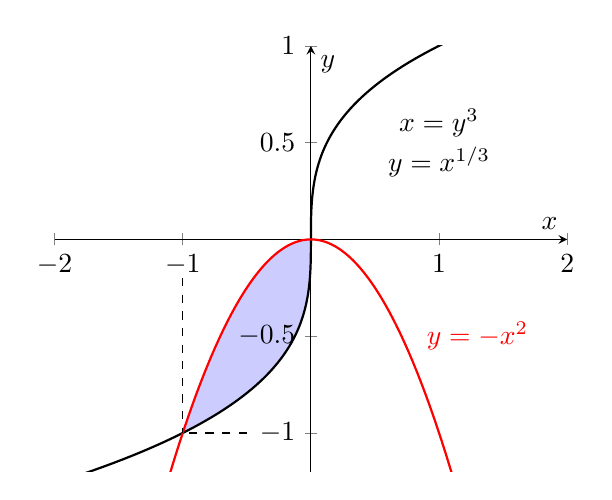
\begin{tikzpicture}
  \begin{axis}[
    axis lines = middle,
    xlabel = {$x$},
    ylabel = {$y$},
    ymin = -1.2, ymax = 1,
    xmin = -2, xmax = 2,
    samples = 200,
    domain = -2:2,
    clip=true,
    scale=0.95,
  ]

  \addplot [
    name path=A,
    domain=-1:0,
    draw=none,
  ] {-x^2};

  \addplot [
    name path=B,
    domain=-1:0,
    draw=none,
  ] ({x^3}, x);

  \addplot [
    fill=blue!20,
  ] fill between[of=A and B];

  \addplot [
    domain=-2:2,
    samples=200,
    thick,
    black,
  ] ({x^3}, x);

  \addplot [
    domain=-2:2,
    samples=200,
    thick,
    red,
  ] {-x^2};

  \draw[dashed] (axis cs:-1,-0.2) -- (axis cs:-1,-1);
  \draw[dashed] (axis cs:-0.5,-1) -- (axis cs:-1,-1);

  \node[red] at (axis cs: 1.3,-0.5) {$y=-x^2$};
  \node at (axis cs: 1,0.6) {$x=y^3$};
  \node at (axis cs: 1,0.4) {$y=x^{1/3}$};

  \end{axis}
\end{tikzpicture}
\end{minipage}
\begin{minipage}{0.5\textwidth}
\begin{align*}
V&=\int_{-1}^0\pi\left[\left(x^{1/3}\right)^2-\left(-x^2\right)^2\right]\,dx\\\\&=\pi\int_{-1}^0\left(x^{2/3}-x^4\right)\,dx\\\\&=\pi\left[\frac35x^{5/3}-\frac{x^5}{5}\right]_{-1}^0\\\\&=\pi\cdot\left[0-\left(-\frac35+\frac15\right)\right]=\boxed{\frac{2\pi}5}
\end{align*}\
\end{minipage}

\end{document}